\documentclass{article}
\usepackage[pdftex]{graphicx,color}
\usepackage[T1]{fontenc}
\usepackage{lmodern}
\usepackage{amsmath}
\usepackage{amsfonts}
\usepackage{subfigure}
\usepackage{textpos}

\usepackage{fullpage}

% be able to use \note environments with a box around the text
\usepackage{fancybox}
\newcommand{\note}[1]{
{\parindent0pt
  \begin{center}
    \shadowbox{
      \begin{minipage}[c]{0.9\linewidth}
        \textbf{Note:} #1
      \end{minipage}
    }
  \end{center}
}}

% use the listings package for code snippets. define keywords for prm files
% and for gnuplot
\usepackage{listings}
\lstset{
  language=C++,
  showstringspaces=false,
  basicstyle=\small\ttfamily,
  columns=fullflexible,
  keepspaces=true,
  frame=single,
  breaklines=true,
  postbreak=\raisebox{0ex}[0ex][0ex]{\hspace{5em}\ensuremath{\color{red}\hookrightarrow\space}}
}
\lstdefinelanguage{prmfile}{morekeywords={set,subsection,end},
                            morecomment=[l]{\#},escapeinside={\%\%}{\%},}
\lstdefinelanguage{gnuplot}{morekeywords={plot,using,title,with,set,replot},
                            morecomment=[l]{\#},}


% use the hyperref package; set the base for relative links to
% the top-level aspect directory so that we can link to
% files in the aspect tree without having to specify the
% location relative to the directory where the pdf actually
% resides
\usepackage[colorlinks,linkcolor=blue,urlcolor=blue,citecolor=blue,baseurl=../]{hyperref}

\newcommand{\dealii}{{\textsc{deal.II}}}
\newcommand{\pfrst}{{\normalfont\textsc{p4est}}}
\newcommand{\trilinos}{{\textsc{Trilinos}}}
\newcommand{\petsc}{{\textsc{PETSc}}}
\newcommand{\aspect}{\textsc{ASPECT}}

\begin{document}
\begin{center}
\textbf{\large{Inner core convection with aspect}}
\end{center}


\vspace{0.2cm}
\textbf{How to run a simulation}
\vspace{0.2cm}

\lstinputlisting[language=prmfile]{cookbooks/inner_core_convection/inner_core_traction.part.6.prm}

To run : "sbatch name-of-bashscript".

\vspace{0.2cm}
\textbf{Governing parameters}
\vspace{0.2cm}

In order to explore the differents regimes of the inner core dynamic, two parameters have to be changed, the Rayleigh number $Ra$, and the phase change number $P$.
The Rayleigh number can directly be changed by adjusting the magnitude of the gravity:
\lstinputlisting[language=prmfile]{cookbooks/inner_core_convection/inner_core_traction.part.2.prm}
The phase change number is implemented as part of the material model, and as a function that can depend on the 
spatial coordinates and/or on time: 
\lstinputlisting[language=prmfile]{cookbooks/inner_core_convection/inner_core_traction.part.1.prm}

\vspace{0.2cm}
\textbf{Mesh refinement}
\vspace{0.2cm}

In the particular case of translation for the inner core convection, a mesh that is finer in the outer boundary is appropriated.
For translation and stable simulations I used:
\lstinputlisting[language=prmfile]{cookbooks/inner_core_convection/inner_core_traction.part.3.prm}

For plume convection simulations :
\lstinputlisting[language=prmfile]{cookbooks/inner_core_convection/inner_core_traction.part.4.prm}

The sum of the "Initial global refinement" and the "Initial adaptative refinement" is always the maximum refinement of the model. In order to have a finest mesh with a refinement of 6 (like for the exemple above), the sum of those two parameters should be 6. The "Initial global refinement" is used to start with an uniform mesh, and then it does a number of mesh refinement step equal to the "Initial adaptive refinement". That means that if the Initial adaptive refinement is setted to 0, the mesh will always be uniform, no matter what is specified elsewhere. Also, in every mesh refinement step, the mesh is only refined or coarsened by one level, respectively. That means that if for example, the start is from an Initial global refinement of 5, the Initial adaptive refinement should be 2, so that refinement levels of 5,6 and 7 are possible (as it's specified in the minimum refinement function). It's also possible to change the fraction of the sphere you want to better define. This can be achieve by changing the first term in the paranthesis, which corresponds to the pourcentage of the sphere you want to define. 

Next step : Use adaptative mesh refinement for the plume convection cases.
 
\vspace{0.2cm}
\textbf{Restart from a previous run}
\vspace{0.2cm}

Some simulations can be very heavy (3D calculations) and thus long. In the particular case of using a server, you could run only limited time simulations and thus need to restart from a previous state.

In order to restart from a previous run:
\lstinputlisting[language=prmfile]{cookbooks/inner_core_convection/inner_core_traction.part.5.prm}
For the first run, "set Resume computation" has to be false and then true if you want to restart from it. Checkpointing files will be created and the number of steps between every checkpoint has to be adjusted.

\vspace{0.4cm}
\textbf{Some results}
\vspace{0.2cm}

Simulations shown on the Figure~\ref{fig:simulations} have been performed with the parameters used above. All of them reached a stationnary state. The regime to which they belong was determined using the paraview visualization tool. A simulation exemple for each regime is shown on the Figure~\ref{fig:inner-core-regimes}. 

\begin{figure}
    \begin{center}
    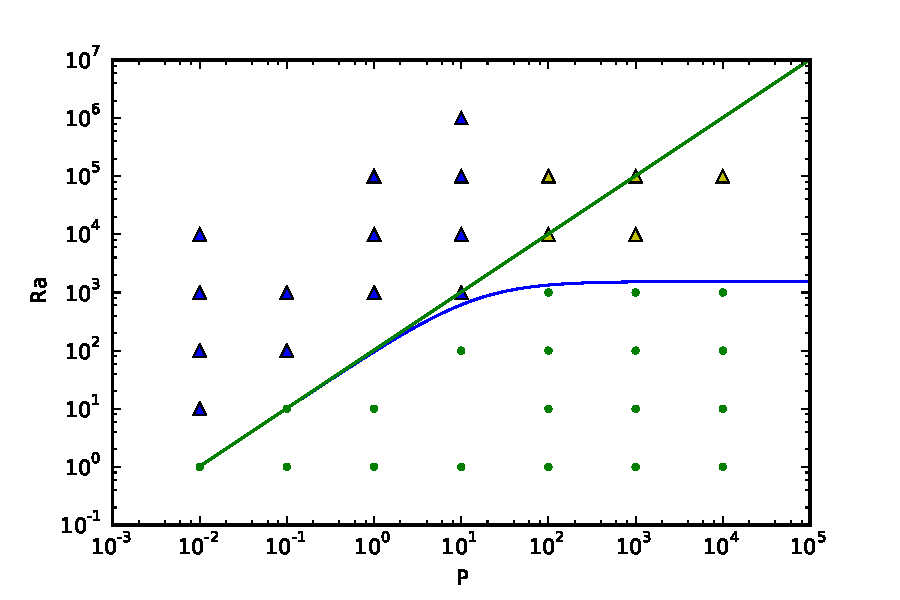
\includegraphics[width=0.6\linewidth]{cookbooks/inner_core_convection/simulations.pdf}
    \caption{Stability diagram for convection in a sphere with phase change at its outer boundary. The stability curves for the first unstable mode (l=1) and the translation are obtained from \cite{Deguen2013}. Triangles are for the convective regimes with, in blue, the translation mode and in yellow, the plume convection mode; points are for the stable cases.}
    \label{fig:simulations}
       \end{center}
\end{figure}

\begin{figure}
    \begin{center}
    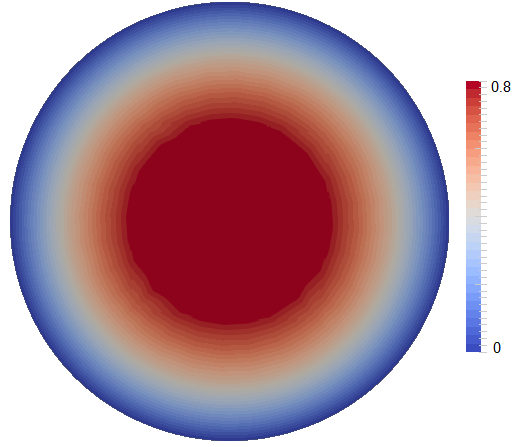
\includegraphics[width=0.25\linewidth]{cookbooks/inner_core_convection/Ra1e0P0rescalemodif.png}
    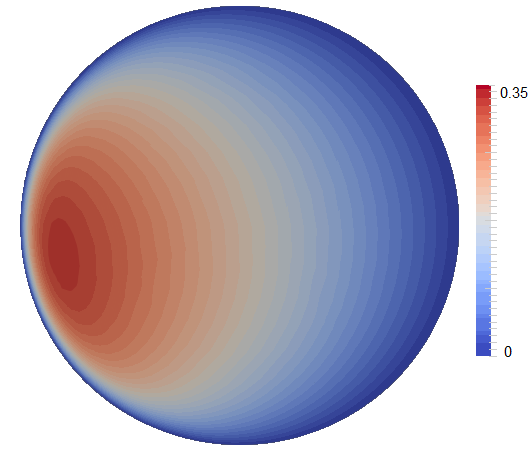
\includegraphics[width=0.25\linewidth]{cookbooks/inner_core_convection/Ra1e2P-1rescalemodif.png}
    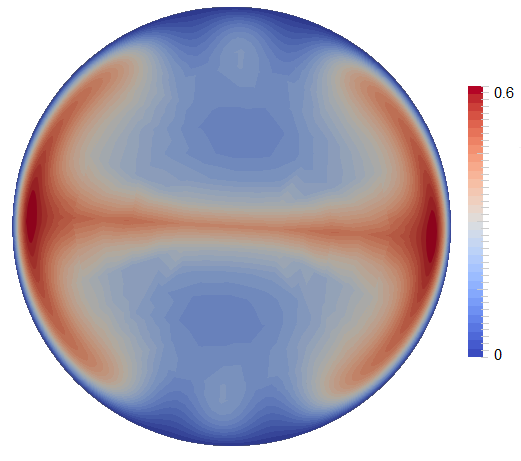
\includegraphics[width=0.25\linewidth]{cookbooks/inner_core_convection/Ra1e5P4rescalemodif.png}
    \caption{Convection regimes in the inner core for different values of $Ra$ and $\mathcal{P}$. From left to right: no convection ($Ra=1, \mathcal{P}=1$), translation ($Ra=10^2, \mathcal{P}=10^{-1}$), plume convection ($Ra=10^5, \mathcal{P}=10^4$).}
    \label{fig:inner-core-regimes}
       \end{center}
\end{figure}

\end{document}